\chapter{Supplementary Material for GPU-accelerated Multi-relational Parallel Graph Retrieval for Web-scale Recommendations}
\label{app:gmpgr}

\section{Pseudo Code of HiPANNS Algorithm}\label{gmpgr:sec:appendix_pseudocode}

This section presents the pseudocodes of the Hierarchically Parallel Approximate Nearest Neighbor Search~(HiPANNS), including inter-candidate HiPANNS~(C-HiPANNS) and inter-query~(Q-HiPANNS).
In Algorithm~\ref{gmpgr:alg:c_hipanns}, inter-candidate HiPANNS~(C-HiPANNS) allows parallel search within the large-scale graph item base to broaden the global search space for more comprehensive retrieval.
In Algorithm~\ref{gmpgr:alg:q_hipanns}, inter-query HiPANNS~(Q-HiPANNS) adaptively aggregates irregular neural computations for more efficient GPU-accelerated retrieval against launch bound from extreme concurrency.



\begin{algorithm}
    \caption{Inter-candidate HiPANNS.}
    \label{gmpgr:alg:c_hipanns}
    \LinesNumbered
    \KwIn{Query user $u$, HNSW $G$, Neighbor hops $T$, heap size $K$, and number of HNSW layers $L$.}
    \KwOut{Top-$K$ retrieved items $V_u$.}
    \Fn{\CHIPANNS{$u$,$G$,$T$,$K$,$L$}}{
        Initialize a $K$-size max heap $\Phi_u$\;
        Initialize $K$ search seeds $S^{(0)}=\{v^{(0)}_{1},v^{(0)}_{2},\cdots,v^{(0)}_{K}\}$ and push them into $\Phi_u$\;
        \For{$l=1,\cdots,L$}{
            Initialize search seeds for $l$-th layer as $S^{(l)}=\Phi_u$\;
            \ForEach{$v^{(l)}_{i} \in S^{(l)}$ in parallel}{
                \For{$t=1,\cdots,T$ in batch}{
                    Retrieve $v^{(l)}_{i}$'s $t$-hop neighbor set $\{v^{(l)}_{i,t_j}\}$\;
                    Calculate the relevance $\delta_{u,v^{(l)}_{i,t_j}}$ by \QHIPANNS{$\{(u,v^{(l)}_{i,t_j})\}$}\;
                    Push $v^{(l)}_{i,t_j}$ into $\Phi_u$\;
                }
            }
        }
        \Return{$\Phi_u$}
    }
\end{algorithm}

\begin{algorithm}
    \caption{Inter-query HiPANNS}
    \label{gmpgr:alg:q_hipanns}
    \LinesNumbered
    \KwIn{GPU cluster $U$, $U$'s batch size $N_U$}
    \KwOut{Relevance values $\delta_{B_i}$}
    \Fn{\QHIPANNS{$B_i$}}{
        Initialize an empty $N_U$-size batch $B_U$ and current batch length $N^{\prime}_U=0$\;
        Initialize a queue $\Psi$\;
        Listen to a batch $B_i=\{(u_{i,1},v_{i,1}),\cdots,(u_{i,N_{B_i}},v_{i,N_{B_i}})\}$ at real-time and push it into $\Psi$\;
        \ForEach{$B_i \in \Psi$}{
            $\epsilon = N_U - N^{\prime}_U$\;
            \eIf{$N_{B_i} \leq \epsilon$}{
                Concentrate batch as $B_U = B_U \cap B_i$ and $N^{\prime}_U = N^{\prime}_U + N_{B_i}$\;
                Calculate $\delta_{B_i}$ on $U$\;
            }{
                Split $B_i$ as $B_i^{[1,\epsilon]}$ and $B_i^{[\epsilon+1,N_{B_i}]}$\;
                Concentrate batch as $B_U = B_U \cap B_i^{[1,\epsilon]}$\;
                Calculate $\delta_{B_i}$ on $U$\;
                Set $B_U = B_i^{[\epsilon+1,N_{B_i}]}$ and $N^{\prime}_U = B_i - \epsilon$\;
            }
        }
        Concentrate $\delta_{B_i}$ if $B_i$ is splited\;
        \Return{$\delta_{B_i}$}
    }
\end{algorithm}


\subsection{Implementation Details}\label{gmpgr:sec:appendix_implementation}

We construct HNSW by $4$ layers consistently for Video, MVideo, Explore, and Fresh datasets. Detailed statistics of layer-wise node numbers in HNSW structures are presented in Table~\ref{gmpgr:tab:nodes}.
Besides, we involve $35$ slots of features in user representation learning.
The neural metric has about $3$ million of learnable parameters.
For commercial online serving, we deploy our methods for $2$ services with $5$ servers, and activate $165$ and $119$ NVIDIA A30 Tensor Core GPUs, respectively. 
Detailed GPU equipment of servers is provided in Table~\ref{gmpgr:tab:gpu}.

\begin{table}[htbp]
    \centering
    \caption{Number of nodes in HNSW layers for four datasets.}
    \label{gmpgr:tab:nodes}
    \begin{tabular}{c|cccc}
        \toprule
         & Video & MVideo & Explore & Fresh \\
        \midrule
        Layer 1 & 281 & 214 & 210 & 78 \\
        Layer 2 & 4,676 & 3,560 & 3,530 & 1,249 \\
        Layer 3 & 79,249 & 61,246 & 60,679 & 20,874 \\
        Layer 4 & 1,335,473 & 1,033,857 & 1,024,531 & 355,585 \\
        \bottomrule
    \end{tabular}
\end{table}

\begin{table}[htbp]
    \centering
    \caption{GPU equipment of five servers for two services.}
    \label{gmpgr:tab:gpu}
    \begin{tabular}{c|ccccc}
        \toprule
         & Server 1 & Server 2 & Server 3 & Server 4 & Server 5 \\
        \midrule
        Service 1 & 28 & 24 & 36 & 40 & 37 \\
        Service 2 & 23 & 15 & 29 & 29 & 23 \\
        \bottomrule
    \end{tabular}
\end{table}






\subsection{Additional Efficiency Analysis}\label{gmpgr:sec:appendix_efficiency}

Here we analyze the efficiency in terms of inference time and search speed on MVideo and Fresh datasets by scattering results of five methods in Figure~\ref{gmpgr:fig:appendix_efficiency}.

\begin{figure}[htbp]
    \centering
    \subfloat[MVideo]{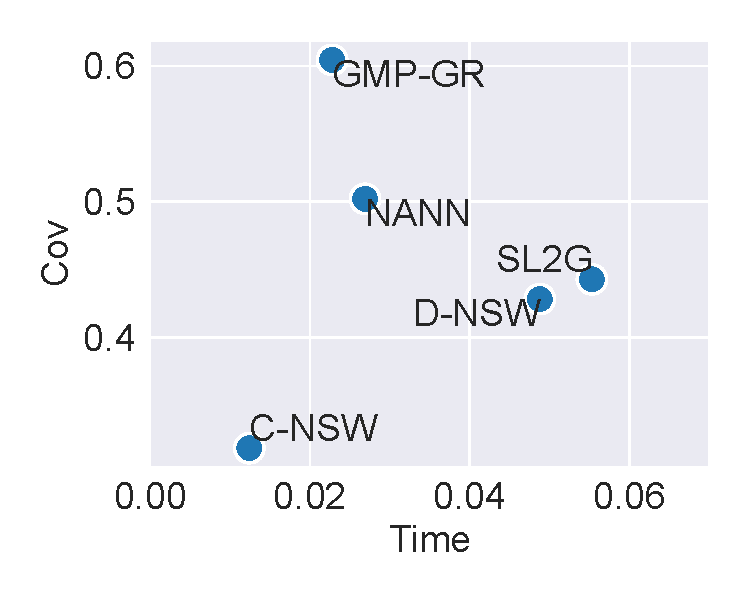
\includegraphics[width=0.48\linewidth]{figures/gmpgr/efficiency_MVideo.pdf}\label{gmpgr:fig:effciency_mvideo}}
    \subfloat[Fresh]{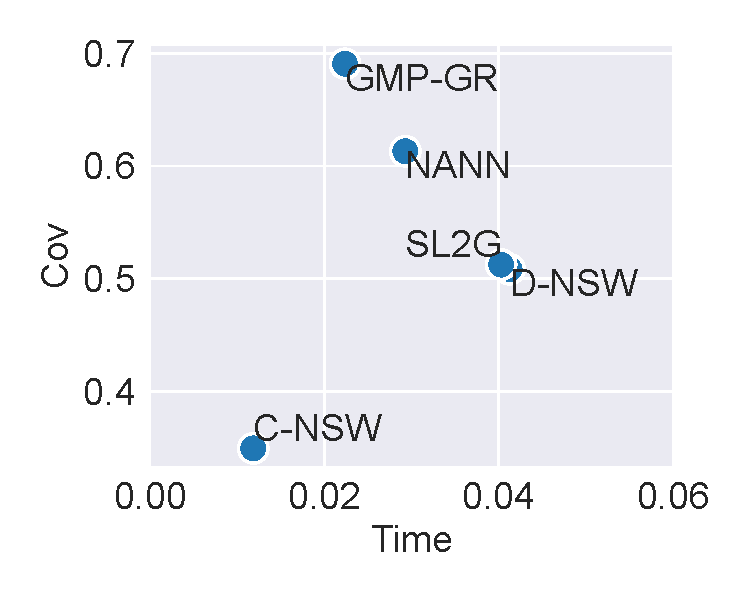
\includegraphics[width=0.48\linewidth]{figures/gmpgr/efficiency_Fresh.pdf}\label{gmpgr:fig:fig:effciency_fresh}}
    \caption{Analysis of correlations between retrieval performance and efficiency on four datasets. Methods close to the left~top~($\nwarrow$) have better retrieval performance, \ie Cov~($\uparrow$), with less time costs~($\leftarrow$).}
    \label{gmpgr:fig:appendix_efficiency}
\end{figure}

\subsection{Additional Ablation Study}\label{gmpgr:sec:appendix_ablation}

In this subsection, we conduct a further ablation study by comparing GMP-GR with GMP-GR-P and GMP-GR-M according to the evaluated results by Rec@10 and Rec@100 in Figure~\ref{gmpgr:fig:appendix_ablation}.

\begin{figure}[htbp]
    \centering
    \subfloat[Rec@10]{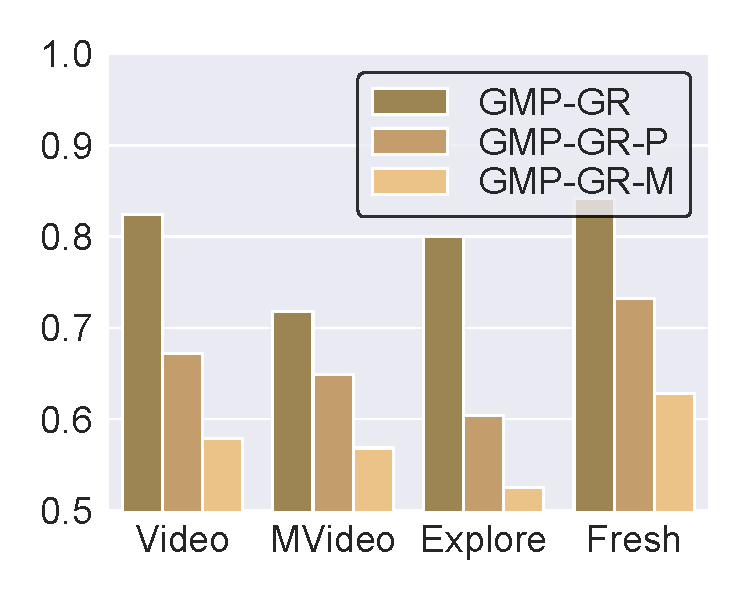
\includegraphics[width=0.48\linewidth]{figures/gmpgr/ablation_Rec10.pdf}\label{gmpgr:fig:ablation_rec10}}
    \subfloat[Rec@100]{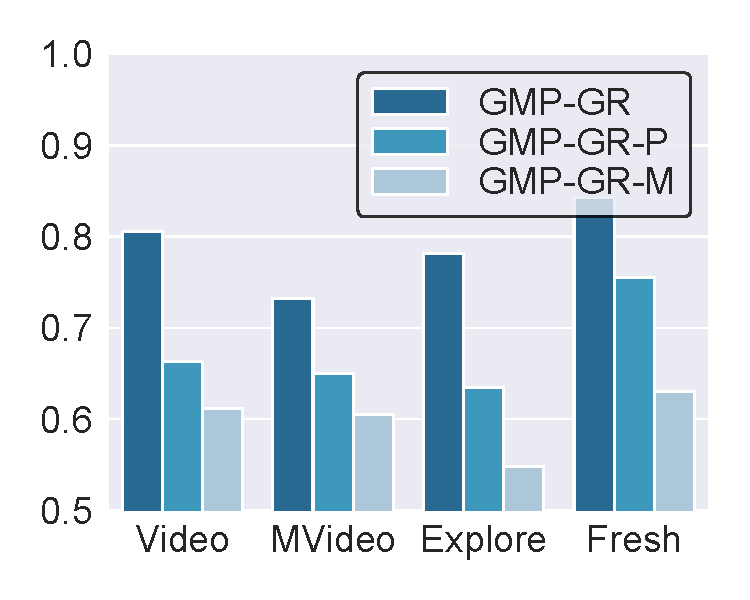
\includegraphics[width=0.48\linewidth]{figures/gmpgr/ablation_Rec100.pdf}\label{gmpgr:fig:ablation_rec100}}
    \caption{Additional ablation study of GMP-GR on retrieval performance~(Rec@10 and Rec@100).}
    \label{gmpgr:fig:appendix_ablation}
\end{figure}
